\documentclass{article}

% I got this template code from https://arxiv.org/abs/1803.04402

\usepackage{amssymb, amsmath, graphicx, subfigure, xparse, array}
\usepackage{physics, authblk}
\usepackage{tikz}
\usepackage{fullpage}
\usepackage{listings}
\usepackage{threeparttable}
\usepackage{physics}
\usepackage{inconsolata}
\usepackage{appendix}
\usepackage[colorlinks=true,linkcolor=black,anchorcolor=black,citecolor=black,filecolor=black,menucolor=black,runcolor=black,urlcolor=black]{hyperref}

\lstdefinelanguage{qwak}{
    keywords=[1]{function, return, if, else, for, in, while},
    keywords=[2]{control, kcontrol, R, measure, dim, zero, swap, true, false},
    keywordstyle=[1]\color{blue},
    keywordstyle=[2]\color{red},
    sensitive=true, % keywords are not case-sensitive
    morecomment=[l]{//}, % l is for line comment
    morecomment=[s]{/*}{*/}, % s is for start and end delimiter
    commentstyle=\color{gray}
}

\lstdefinelanguage{liquid}{
    keywords={let, for, in, do},
    morekeywords=[2]{CNOT,M},
    keywordstyle=\color{blue},
    keywordstyle=[2]\color{red},
    sensitive=true, % keywords are not case-sensitive
    morecomment=[l]{//}, % l is for line comment
    morecomment=[s]{/*}{*/}, % s is for start and end delimiter
    morestring=[b]", % defines that strings are enclosed in double quotes
}

\lstset{
  basicstyle=\ttfamily,
  language=Qwak
}

\usetikzlibrary{shapes,arrows}

% Define block styles
\tikzstyle{block} = [rectangle, draw, 
    text centered, rounded corners, minimum height=4em]
\tikzstyle{line} = [draw, -latex']

\setlength\extrarowheight{2pt}

\begin{document}

%
%
\title{Qwak \\ A New Quantum Programming Language}
\author[1]{Gabriel Stella}
\author[1]{Jonathan Beechner}
\affil[1]{\small \textit{Department of Computer Science, \protect\\ Texas A\&M University, College Station}}
\date{}

\maketitle

\begin{abstract}
We introduce the Qwak quantum programming language, its design process, and related components. Qwak is a simple, intuitive language for higher-level quantum programming. As opposed to previous work, it attempts to separate the domains of quantum and classical programming by allowing the user to interact with the Qwak system through any classical language of their choice; in this way, Qwak is a \textit{quantum-first} programming language.
\end{abstract}



\section{Introduction}

While quantum computers are currently difficult to implement physically, progress is being made in engineering quantum computers with more and more qubits. However, modern quantum programming languages are lacking in several ways. Most notably, Quipper allows the programmer to write invalid quantum programs, while Q\# is simply quantum-enabled classical computing. In this project, we developed Qwak, a programming language that focuses solely on quantum computation in order to remain simple and intuitive, leaving classical computation to a language of the programmer’s choice.

\section{Qwak and its Components}

This project involved the design of the Qwak language and the implementation of three projects: first, the Qwality C++ quantum simulator; second, a C++ implementation of a Qwak parser and runtime environment; third, a command-line Qwak interpreter called Qwaket. The state of these projects can be viewed on our GitHub repository at \url{https://github.com/GabrielRStella/Qwak}.

\subsection{Qwality}

Qwality is a simple C++ library for quantum simulation. It currently supports the quantum circuit model of computation with pure quantum state vectors. While it supports realistic quantum functionality, e.g. mutable quantum state operations, it also supports a wide variety of simulation-enabled functions such as state cloning, measurement without state collapse, and more. It is based on the GiNaC C++ library for symbolic computation, allowing expressions to be represented with perfect accuracy.

\subsection{Qwak}

Qwak is a simple language for quantum computation. It is designed to be an intuitive \textit{quantum-first} language that does not attempt to provide extensive classical computation abilities. In order to bridge this gap, Qwak can be controlled from a classical language of the user’s choice, or from the Qwaket interactive shell.

The current implementation of Qwak relies on a C++ runtime environment, which links directly to the Qwality simulator. However, our goal for the future design of Qwak is for compilation of Qwak programs to be done in two stages, as seen in Figure \ref{fig:comp-stages}. The first stage compiles a Qwak program to a simpler intermediate format, similar to bytecode. The second state compiles this intermediate code to a quantum assembly language, such as QASM. The motivation for this two-stage process is that Qwak allows for variables, control flow, functions, and other high-level language constructs that a quantum assembly language may not. The intermediate language, while simpler for a program to compile, must still support these features in some limited way. Thus, the process of compiling this intermediate language can actually be seen as taking a quantum program, along with user-given variable values, to generate a fixed quantum circuit.

\begin{figure}[h]
\centering
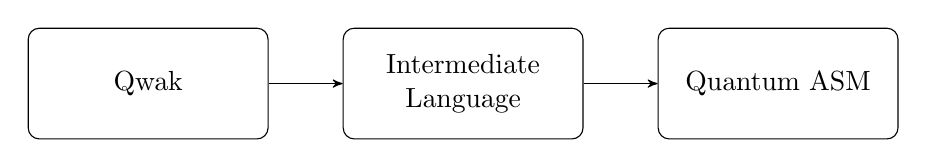
\begin{tikzpicture}[line/.style={->, >=stealth', every node/.style={fill=white}}]
\node [block, text width=8em] at (0,0) (qwak) {Qwak};
\node [block, text width=8em] at (4,0) (intermediate) {Intermediate Language};
\node [block, text width=8em] at (8,0) (asm) {Quantum ASM};

\draw [line] (qwak) -- (intermediate);
\draw [line] (intermediate) -- (asm);
\end{tikzpicture}
\caption{Qwak compilation stages} \label{fig:comp-stages}
\end{figure}

The ASM itself can then be run on a quantum computer or using a quantum simulator; the Qwak system would not require any knowledge of its use. The separation of the compilation into two stages may also make it easier for interactive shell utilities like Qwaket to be implemented.

As stated before, Qwak is meant to be controlled by a classical programming language. For this to be done, the classical programming language requires a library that can interact with a quantum computer (or simulator) to execute quantum assembly code; it then also requires in-language bindings for compiling Qwak code to quantum assembly to instantiate and execute a circuit. The process of classical control is depicted in Figure \ref{fig:info-flow}, where the Quantum Runtime may be a simulator or a quantum computer.

\begin{figure}[h]
\centering
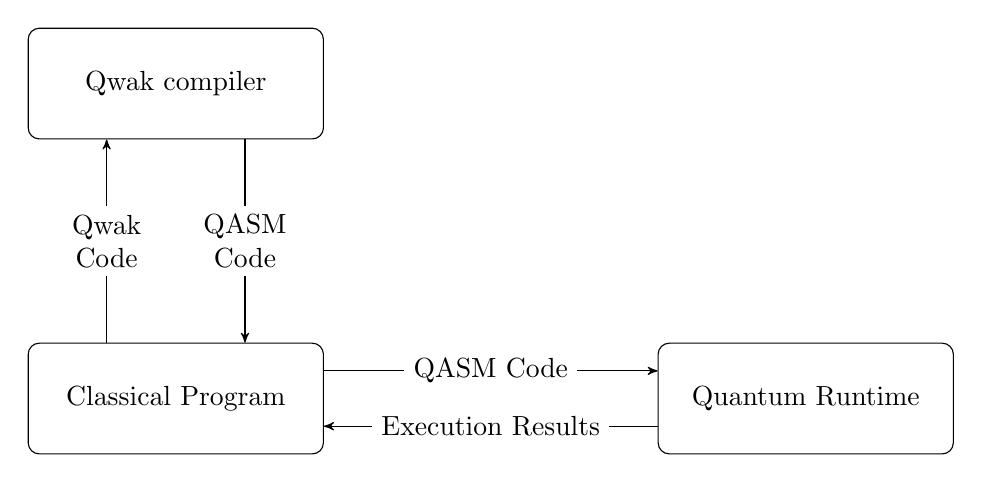
\begin{tikzpicture}[line/.style={->, >=stealth', every node/.style={fill=white}}]
\node [block, text width=10em] at (0,0) (compiler) {Qwak compiler};
\node [block, text width=10em] at (0,-4) (program) {Classical Program};
\node [block, text width=10em] at (8,-4) (runtime) {Quantum  Runtime};

\draw [line] ([xshift=-2.5em] program.north) -- node[align=center] {Qwak\\Code} ([xshift=-2.5em] compiler.south);
\draw [line] ([xshift=2.5em] compiler.south) -- node[align=center] {QASM\\Code} ([xshift=2.5em]
program.north);

\draw [line] ([yshift=1em] program.east) -- node {QASM Code} ([yshift=1em] runtime.west);
\draw [line] ([yshift=-1em] runtime.west) -- node {Execution Results} ([yshift=-1em] program.east);
\end{tikzpicture}
\caption{Qwak information flow} \label{fig:info-flow}
\end{figure}

Figure \ref{fig:lang-comparison} shows two short code snippets comparing another quantum programming framework, LIQUi$\ket{}$, to Qwak. We aimed to make Qwak simple and intuitive to those who have worked with quantum algorithms. Its goal is to be a truly quantum language, as opposed to a classical language with quantum capabilities. More details on the Qwak language can be found in the appendices.

\begin{figure}
\noindent\hspace*{\fill}\begin{minipage}[t]{.4\textwidth}
\centerline{LIQUi$\ket{}$}
\begin{lstlisting}[frame=tlrb,language=liquid]{Name}
let Entangle1(entSiz:int) =
  let ket = Ket(entSiz)
  let _ = ket.Single()
  let qs = ket.Qubits
  H qs
  let q0 = qs.Head
  for i in 1..qs.Length-1 do
    let q = qs.[i]
    CNOT[q0;q]
  M >< qs
\end{lstlisting}
\end{minipage}\hfill
\begin{minipage}[t]{.4\textwidth}
\centerline{Qwak}
\begin{lstlisting}[frame=tlrb]{Name}
function entangle(n) {
  state = |0^n>
  H(state)[0]
  xx = X^**(n-1)
  cx = control(xx)
  cx(state)
  return measure(state)
}
\end{lstlisting}
\end{minipage}\hspace*{\fill}
\caption{Entangling $n$ qubits in LIQUi$\ket{}$ and Qwak.} \label{fig:lang-comparison}
\end{figure}

\subsection{Qwaket}

The Qwaket command-line shell, based on our Qwality simulation library, allows the user to interactively experiment with Qwak programming via line-by-line execution and Qwak file parsing. It also supports several convenience features for testing such as the ability to print the global quantum state, the list of variables, and the list of loaded functions. Qwaket currently comes with ``stl.qwak'', which demonstrates some basic features of the Qwak language.

\section{Future Work}

There are two general classes of work to be done on the Qwak project. The first relates to the Qwak language; as discussed more in Appendix \ref{sec:langdef}, the Qwak language is currently not fully expressive, and more work needs to be done to support more general programs. We also currently have no specification for the Qwak intermediate language. The second class of improvements is to the implementation of Qwality and Qwak.

\subsection{Qwality}

\subsubsection{Improved symbolic algebra computations}

Qwality currently uses the GiNaC C++ library for symbolic computation. While it is useful, the library has drawbacks when applied to quantum computation; for example, it is not able to properly simplify very common quantum expressions involving $e^{i\theta}$. We would like to implement a quantum-specific symbolic math library that will enable better handling of the terms that often appear in quantum algorithms.

\subsubsection{Noise simulation}
Physical implementations of quantum computers experience complicated errors at every step of computation. However, our simulator preserves perfect precision by using symbolic expressions. In future work, artificial noise may be an optional feature of our quantum simulator to help programmers experiment with a more realistic scenario.

\subsection{Qwak}

The current Qwak implementation is a basic prototype that relies fully on the Qwality simulation library; a proper implementation must be made that follows the compilation process outlined previously in this paper.

\subsection{Other Work}

\subsubsection{Qubit sharing}

In future work, we would like to explore the possibility of shared quantum programming; that is, programming ``circuits'' that span some nontrivial geographic distance, including simulations that run between several computers. This could allow better experimentation with quantum teleportation, super dense coding, and quantum cryptography. This could be facilitated by a quantum state server that allows users to interact with a small substate of the globally-shared quantum state.





\appendixpage
\appendix

\section{Qwality Overview}
\label{sec:qwality-overview}

The Qwality simulation library is composed of two C++ classes: \lstinline$QuantumState$ and \lstinline$QuantumGate$. As a general design principle, Qwality supports both in-place (marked with an underscore in the source) and out-of-place operations on all objects. For a complete list of supported functions, refer to the Qwak GitHub repository.

\subsection{QuantumState}

The QuantumState class represents an $n$-qubit quantum state vector. All qubits within a \lstinline$QuantumState$ are fully connected, and \lstinline$QuantumState$ objects can be combined via the tensor product.

\lstinline$QuantumState$ objects support a general group of important operations: measurement (including partial measurement), tensor product, and gate application. All of these operations include in-place (mutating) and out-of-place (cloning) versions.

One important feature of \lstinline$QuantumState$ is the \lstinline$applyPartial$ function. This allows the programmer to apply an $m$-qubit gate to a substate of an $n$-qubit state, where $n>m$, without having to tensor the gate with the identity matrix $n-m$ times. This function also includes automatic swapping of qubits given the programmer’s desired order of application.

\subsection{QuantumGate}

A Qwality \lstinline$QuantumGate$ is simply a square matrix with support for typical quantum functions: tensor product, gate concatenation, inverse, and conjugate transpose. Most importantly, the \lstinline$QuantumGate$ class provides static functions for creating some common quantum gates:

\begin{center}
\begin{tabular}{| l | l |}
\hline
\lstinline$I$ & The single-qubit identity operation. \\ \hline
\lstinline$H$ & The single-qubit Hadamard gate. \\ \hline
\lstinline$X$ & The single-qubit Pauli $X$ gate. \\ \hline
\lstinline$Y$ & The single-qubit Pauli $Y$ gate. \\ \hline
\lstinline$Z$ & The single-qubit Pauli $Z$ gate. \\ \hline
\lstinline[language=C]$R(k)$ & The single-qubit phase rotation gate $R_k$. \\ \hline
\lstinline[language=C]$control(U)$ & Creates a quantum boolean-controlled gate from the unitary $U$. \\ \hline
\lstinline[language=C]$kcontrol(U, m)$ & Creates the integer-controlled gate $C_m(U)$. \\ \hline
\lstinline[language=C]$swap(qubits)$ & Creates a swap gate using the given vector of positions. \\ \hline
\lstinline$makeUnitary(f)$ & Creates a reversible unitary from the given classical function. \\ \hline

\end{tabular}
\end{center}

\pagebreak

\section{Qwak Language Definition}
\label{sec:langdef}

\subsection{Types}

QWAK currently supports 3 types: quantum state references, quantum gates, and integer values. In the future, we will work on the integration of classical states, list types, and arbitrary scalar expressions.

\begin{center}
\begin{threeparttable}[b]
\begin{tabular}{| l | l |}
\hline
\multicolumn{2}{|c|}{\textbf{Types}} \\ \hline
\lstinline!x = |0>! & A quantum state variable. \\ \hline
\lstinline!U = H! & A quantum gate variable. \\ \hline
\lstinline!n = 5! & An integer variable. \\ \hline
\multicolumn{2}{|c|}{\textbf{Future\tnote{1}}} \\ \hline
\lstinline!c = |0>! & A classical state variable. \\ \hline
\lstinline!xs = [|0>, |1>]! & A list variable. \\ \hline
\lstinline!ns = [0, 3..6, n..m]! & A list variable defined using ranges. \\ \hline
\end{tabular}
\begin{tablenotes}
\item [1] It is not decided how these will be integrated into the language as of yet. Thus, there may be some ambiguity right now.
\end{tablenotes}
\end{threeparttable}
\end{center}

\subsection{Boolean Values}
The truth value of a QWAK variable is essentially like an override of the C++ operator bool(). It is used for things like while loops.

\begin{center}
\begin{tabular}{| l | l |}
\hline
\multicolumn{2}{|c|}{\textbf{Boolean Values}} \\ \hline
Quantum state & Always true. \\ \hline
Quantum gate & Always true. \\ \hline
Integer (or scalar) \lstinline!n! & True if \lstinline$n != 0$. \\ \hline
Classical state \lstinline!c! & True if \lstinline!c == |1>! (or \lstinline$c != |0^n>$ for \lstinline!n!-bit states). \\ \hline
List \lstinline!ls! & True if \lstinline$dim(ls) != 0$. \\ \hline
\end{tabular}
\end{center}

\subsection{Variables}

Variables in QWAK have a type, however they are not \textit{explicitly} typed; variables are created at their first assignment, and deleted when out of scope. Their type is based on the type of their most recent assignment, and can change at any time.

\begin{center}
\begin{tabular}{| l | m{7cm} |}
\hline
\multicolumn{2}{|c|}{\textbf{Variables}} \\ \hline
\begin{lstlisting}
x = |0>
x = H
\end{lstlisting} & Example of a variable’s initial assignment, to type \textit{quantum state}, and subsequent reassignment to type \textit{quantum gate}. \\ \hline
\multicolumn{2}{|c|}{\textbf{Default Variables}} \\ \hline
\lstinline$I$ & Single-qubit identity operator. \\ \hline
\lstinline$H$ & Single-qubit Hadamard gate. \\ \hline
\lstinline$X$ & Single-qubit Pauli $X$ gate. \\ \hline
\lstinline$Y$ & Single-qubit Pauli $Y$ gate. \\ \hline
\lstinline$Z$ & Single-qubit Pauli $Z$ gate. \\ \hline
\lstinline$STATE$ & A pseudo-variable that represents the program’s entire quantum state. \\ \hline
\end{tabular}
\end{center}

\pagebreak

\subsection{Functions}

Functions in QWAK are identified by their name, their argument list (count and names), and whether they take a secondary argument of a list of qubits. See Appendix C for more examples.

\begin{center}
\begin{tabular}{| l | l |}
\hline
\multicolumn{2}{|c|}{\textbf{Functions}} \\ \hline
\begin{lstlisting}
function name(args)[qubits] {
  //function body
}
\end{lstlisting} & General form of a QWAK function. \\ \hline
\end{tabular}
\end{center}

\subsection{Built-in Operators}

Builtin operators work just like other QWAK functions, except that they are supported by the QWAK runtime.

\begin{center}
\begin{tabular}{| l | m{8cm} |}
\hline
\multicolumn{2}{|c|}{\textbf{Functions}} \\ \hline
\begin{lstlisting}
dim(x)
dim(U)
dim(n)
dim(c)
dim(xs)
\end{lstlisting} & 
Retrieves the dimensionality of the given object. The returned value is an integer. \\ \hline
\begin{lstlisting}
measure(x)
measure(x)[qubits]
\end{lstlisting} & 
Measures a substate of the quantum state \lstinline$x$, in the given order. The measured value is returned as a classical state, and the measured substate of \lstinline$x$ is collapsed. \\ \hline
\begin{lstlisting}
zero(x)
zero(x)[qubits]
\end{lstlisting} & 
Has the effect as if calling \lstinline$measure(x)$, but the result is always \lstinline$0$; essentially restores the given substate of \lstinline$x$ to \lstinline$0$. \\ \hline
\begin{lstlisting}
swap(ns)
\end{lstlisting} & 
Creates a swap gate based on the integer arguments in the list \lstinline$ns$. The returned gate \lstinline$U$ will be such that \lstinline$dim(U) == dim(ns)$. The swap is constructed so that the \lstinline$i$-th qubit inputted will be swapped to the \lstinline$ns[i]$ position in the output. \\ \hline
\begin{lstlisting}
control(U)
control(U, i)
\end{lstlisting} & 
Returns a single-qubit controlled version of the quantum gate \lstinline$U$ such that the \lstinline$i$-th qubit of the returned gate is the control qubit. \\ \hline
\begin{lstlisting}
kcontrol(U, m)
\end{lstlisting} & 
Returns an integer-controlled version of \lstinline$U$ with \lstinline$m$ control qubits. The control qubits will be the first \lstinline$m$ qubits of the returned gate. \\ \hline
\begin{lstlisting}
R(k)
\end{lstlisting} & 
Returns the phase rotation gate $R_k$, where $k$ is an integer. \\ \hline
\end{tabular}
\end{center}

\pagebreak

\subsection{Statements}

Statements form the body of a QWAK function. There are several different types.

\begin{center}
\begin{tabular}{| l | m{8cm} |}
\hline
\multicolumn{2}{|c|}{\textbf{Statements}} \\ \hline
\begin{lstlisting}
return expression
\end{lstlisting} & A return statement. There should be at most one per function, and no other statements after it. \\ \hline
\begin{lstlisting}
expression
identifier = expression
\end{lstlisting} & An assignment. The actual assignment is optional, while the expression is not; many meaningful operations, such as quantum gate application, have no need for an assignment. \\ \hline
\begin{lstlisting}
if expression {
  //if body
}
\end{lstlisting} & A simple \textit{if} statement. The body is executed if expression evaluates to \lstinline$true$. \\ \hline
\begin{lstlisting}
if expression {
  //if body
} else {
  //else body
}
\end{lstlisting} & A simple \textit{if-else} statement. If expression evaluates to \lstinline$true$, the \textit{if body} is executed; otherwise, the \textit{else body} is executed. \\ \hline
\begin{lstlisting}
for identifier in expression {
  //for body
}
\end{lstlisting} & A simple \textit{for} loop over each element in the result of \lstinline$expression$. Note this implies that \lstinline$expression$ should evaluate to a list. \\ \hline
\begin{lstlisting}
while expression {
  //while body
}
\end{lstlisting} & A simple \textit{while} loop. Will execute as long as \lstinline$expression$ evaluates to \lstinline$true$ (according to the truth value of its result). \\ \hline
\end{tabular}
\end{center}

A note on statement groups: While the above definitions include curly braces, QWAK should treat a statement group (list of statements within curly braces) as its own type of statement, so that the control structures replace {body} with some arbitrary statement, which may or may not be a group. This opens up more flexibility in the way code is written.

\subsection{Expressions}

\begin{center}
\begin{tabular}{| l | m{11cm} |}
\hline
\multicolumn{2}{|c|}{\textbf{Expressions}} \\ \hline
\multicolumn{2}{|c|}{Binary Operators} \\ \hline
\lstinline$+$ & Scalar addition (or list concatenation) \\ \hline
\lstinline$-$ & Scalar subtraction \\ \hline
\lstinline$*$ & Multiplication; works on scalars or quantum gates (gate concatenation = matrix multiplication). Both operands must be of the same type. \\ \hline
\lstinline$/$ & Scalar division \\ \hline
\lstinline$^$ & State concatenation, e.g. \lstinline$|0^n>$ \\ \hline
\lstinline$**$ & Exponent; right-hand operand must be a scalar. Left-hand operand may be a scalar or matrix. \\ \hline
\lstinline$^*$ & Tensor product; works on quantum gates or quantum states. When two quantum state references are the input, this simply returns the combination of both states. \\ \hline
\lstinline$^**$ & Tensor exponent. Due to the no-cloning theorem, this is only supported by quantum gates. The right-hand operand should be an integer. \\ \hline
\lstinline$==$ & Equality. Both operands must be of the same type. The equality expression will evaluate to a scalar; if true, \lstinline$1$, else \lstinline$0$. This means that the truth value of \lstinline$(a == b)$ is the same as whether \lstinline$a$ equals \lstinline$b$. While this isn’t technically allowed for quantum states, a Qwak implementation may or may not allow equality checks of arbitrary quantum states. \\ \hline
\multicolumn{2}{|c|}{Other} \\ \hline
\begin{lstlisting}
x[qubits]
c[bits]
\end{lstlisting} & State subscript; returns another (smaller) state. qubits and bits must be integer-valued lists. \\ \hline
\begin{lstlisting}
xs[pos]
\end{lstlisting} & List subscript. Returns a single value. \\ \hline
\begin{lstlisting}
U(x)
U(x)[qubits]
\end{lstlisting} & Gate application. Applies the gate \lstinline$U$ to the given qubits (in order) of state \lstinline$x$. If qubits is not given, \lstinline$U$ is applied (in default order) to the entirety of \lstinline$x$. \\ \hline
\begin{lstlisting}
example(args)
example(args)[qubits]
\end{lstlisting} & Applies the function example to the list of arguments given in its parentheses. An optional secondary argument of an integer list can be placed directly after the parentheses, just like with a quantum gate application. If qubits is not given, it is as if an empty list is passed as the secondary argument. \\ \hline
\end{tabular}
\end{center}

\subsection{Representation of Quantum States}

The Qwak runtime has several large quantum states in the background. When new qubits are created for a variable assignment, a new quantum state is created, the qubits are put into that state, and a reference to the state is returned. Any quantum state referenced from then on will be a substate of that state or other states. These backend quantum states can be tensored and untensored. The mechanisms for the user (programmer) to do this are not clear yet; the current implementation of Qwak only supports a single backend quantum state, with no untensoring.

This makes it clear why operations such as tensoring two states are trivial: if each substate is represented by a list of qubits, then the tensor product of two states is simply the concatenation of their lists.

\subsection{Storage of Variables}

The only real data in a QWAK program is the underlying quantum state and any quantum gates. Variables can all be seen as references into this “pool” of actual information. Thus, all variables are essentially pointers (with some extra information), and they can be passed by value and created/deleted using simple scope rules. Note that this would however mean that lists would have to become part of the pool; we could probably use some simple reference-counting pointers to handle list garbage collection.

\section{Qwak Code Snippets}
\label{sec:code-snippets}

The following snippets show some ideal QWAK code, along with its meaning. Note that these snippets are for clarity; some could be condensed or simplified.

\begin{center}
\begin{tabular}{| l | m{8cm} |}
\hline
\begin{lstlisting}
function KetPlus() {
  return H(|0>)
}
\end{lstlisting} & Creates and returns the single-qubit state $\ket +$. \\ \hline
\begin{lstlisting}
function Bell() {
  s = |00>
  cx = control(X)
  H(s)[0]
  cx(s)
  return s
}
\end{lstlisting} & Creates and returns the bell state $\ket{\phi +}$. \\ \hline
\begin{lstlisting}
function Deutsch(U) {
  x=|01>
  hh = H^*H
  hh(x)
  U(x)
  hh(x)
  return measure(x)[0]
}
\end{lstlisting} & Runs Deutsch’s algorithm on the given single-qubit unitary $U_f$, returning classical $\ket 0$ if $f$ is constant and $\ket 1$ if $f$ is balanced. \\ \hline
\begin{lstlisting}
function Deutsch(U) {
  x=|01>
  hh = H^*H
  (hh * U * hh)(x)
  return measure(x)[0]
}
\end{lstlisting} & Alternate implementation of the above. Demonstrates application of a quantum gate that is the result of an expression. \\ \hline
\begin{lstlisting}
function Entangle(n) {
  x = |0^n>
  H(x)[0]
  xx = X^**(n-1)
  cx = control(xx)
  cx(x)
  return x
}
\end{lstlisting} & Entangles $n$ qubits into the state $\frac{1}{\sqrt 2}\left(\ket{0^n}+\ket{1^n}\right)$. \\ \hline
\begin{lstlisting}
function Entangle(n) {
  x = |0^n>
  first = x[0]
  H(first)
  cx = control(X^**(n-1))
  return cx(x)
}
\end{lstlisting} & Alternate implementation of the above. Demonstrates that the value returned by a quantum gate application is the substate that it acted on. \\ \hline

\end{tabular}
\end{center}

\end{document}
